\documentclass[authoryear,preprint]{sigplanconf}

\usepackage{amsmath}
\usepackage{tikz}

%vim: set makeprg=runghc make:

%% ODER: format ==         = "\mathrel{==}"
%% ODER: format /=         = "\neq "
%
%
\makeatletter
\@ifundefined{lhs2tex.lhs2tex.sty.read}%
  {\@namedef{lhs2tex.lhs2tex.sty.read}{}%
   \newcommand\SkipToFmtEnd{}%
   \newcommand\EndFmtInput{}%
   \long\def\SkipToFmtEnd#1\EndFmtInput{}%
  }\SkipToFmtEnd

\newcommand\ReadOnlyOnce[1]{\@ifundefined{#1}{\@namedef{#1}{}}\SkipToFmtEnd}
\usepackage{amstext}
\usepackage{amssymb}
\usepackage{stmaryrd}
\DeclareFontFamily{OT1}{cmtex}{}
\DeclareFontShape{OT1}{cmtex}{m}{n}
  {<5><6><7><8>cmtex8
   <9>cmtex9
   <10><10.95><12><14.4><17.28><20.74><24.88>cmtex10}{}
\DeclareFontShape{OT1}{cmtex}{m}{it}
  {<-> ssub * cmtt/m/it}{}
\newcommand{\texfamily}{\fontfamily{cmtex}\selectfont}
\DeclareFontShape{OT1}{cmtt}{bx}{n}
  {<5><6><7><8>cmtt8
   <9>cmbtt9
   <10><10.95><12><14.4><17.28><20.74><24.88>cmbtt10}{}
\DeclareFontShape{OT1}{cmtex}{bx}{n}
  {<-> ssub * cmtt/bx/n}{}
\newcommand{\tex}[1]{\text{\texfamily#1}}	% NEU

\newcommand{\Sp}{\hskip.33334em\relax}


\newcommand{\Conid}[1]{\mathit{#1}}
\newcommand{\Varid}[1]{\mathit{#1}}
\newcommand{\anonymous}{\kern0.06em \vbox{\hrule\@width.5em}}
\newcommand{\plus}{\mathbin{+\!\!\!+}}
\newcommand{\bind}{\mathbin{>\!\!\!>\mkern-6.7mu=}}
\newcommand{\rbind}{\mathbin{=\mkern-6.7mu<\!\!\!<}}% suggested by Neil Mitchell
\newcommand{\sequ}{\mathbin{>\!\!\!>}}
\renewcommand{\leq}{\leqslant}
\renewcommand{\geq}{\geqslant}
\usepackage{polytable}

%mathindent has to be defined
\@ifundefined{mathindent}%
  {\newdimen\mathindent\mathindent\leftmargini}%
  {}%

\def\resethooks{%
  \global\let\SaveRestoreHook\empty
  \global\let\ColumnHook\empty}
\newcommand*{\savecolumns}[1][default]%
  {\g@addto@macro\SaveRestoreHook{\savecolumns[#1]}}
\newcommand*{\restorecolumns}[1][default]%
  {\g@addto@macro\SaveRestoreHook{\restorecolumns[#1]}}
\newcommand*{\aligncolumn}[2]%
  {\g@addto@macro\ColumnHook{\column{#1}{#2}}}

\resethooks

\newcommand{\onelinecommentchars}{\quad-{}- }
\newcommand{\commentbeginchars}{\enskip\{-}
\newcommand{\commentendchars}{-\}\enskip}

\newcommand{\visiblecomments}{%
  \let\onelinecomment=\onelinecommentchars
  \let\commentbegin=\commentbeginchars
  \let\commentend=\commentendchars}

\newcommand{\invisiblecomments}{%
  \let\onelinecomment=\empty
  \let\commentbegin=\empty
  \let\commentend=\empty}

\visiblecomments

\newlength{\blanklineskip}
\setlength{\blanklineskip}{0.66084ex}

\newcommand{\hsindent}[1]{\quad}% default is fixed indentation
\let\hspre\empty
\let\hspost\empty
\newcommand{\NB}{\textbf{NB}}
\newcommand{\Todo}[1]{$\langle$\textbf{To do:}~#1$\rangle$}

\EndFmtInput
\makeatother
%

\begin{document}

%\conferenceinfo{WXYZ '05}{date, City.} 
%\copyrightyear{2005} 
%\copyrightdata{[to be supplied]} 

%\titlebanner{banner above paper title}        % These are ignored unless
%\preprintfooter{short description of paper}   % 'preprint' option specified.

\title{Matrices! Of Types!}
%\subtitle{Subtitle Text, if any}

\authorinfo{Dan Piponi}
           {Google}
           {dpiponi\text{\tt gmail\char46{}com\char125{}~\char92{}authorinfo\char123{}Brent~Yorgey\char125{}~~~~~~~~~~~~\char123{}University~of~Pennsylvania\char125{}~~~~~~~~~~~~\char123{}byorgey}cis.upenn.edu}

\maketitle

\begin{abstract}
Matrices of types are sweet
\end{abstract}

%\category{CR-number}{subcategory}{third-level}

%\terms
%term1, term2

%\keywords
%matrices, types

\section{Introduction}

\begin{itemize}
\item Problem statement: how to constrain the leaves of a type to
  conform to a regular expression?

\item Maybe show an ad-hoc solution to a special case, to give a
  better sense of the problem.

I'm listing some elementary examples. We don't have to use all of them.

Ordinary lists:
\begingroup\par\noindent\advance\leftskip\mathindent\(
\begin{pboxed}\SaveRestoreHook
\column{B}{@{}>{\hspre}l<{\hspost}@{}}%
\column{3}{@{}>{\hspre}l<{\hspost}@{}}%
\column{E}{@{}>{\hspre}l<{\hspost}@{}}%
\>[3]{}\mathbf{data}\;\Conid{List}\;\Varid{a}\mathrel{=}\Conid{Nil}\mid \Conid{Cons}\;\Varid{a}\;(\Conid{List}\;\Varid{a}){}\<[E]%
\ColumnHook
\end{pboxed}
\)\par\noindent\endgroup\resethooks
Lists with alternating elements:
\begingroup\par\noindent\advance\leftskip\mathindent\(
\begin{pboxed}\SaveRestoreHook
\column{B}{@{}>{\hspre}l<{\hspost}@{}}%
\column{3}{@{}>{\hspre}l<{\hspost}@{}}%
\column{E}{@{}>{\hspre}l<{\hspost}@{}}%
\>[3]{}\mathbf{data}\;\Conid{AList}\;\Varid{a}\;\Varid{b}\mathrel{=}\Conid{ANil}\mid \Conid{ACons}\;\Varid{a}\;(\Conid{BList}\;\Varid{a}\;\Varid{b}){}\<[E]%
\\
\>[3]{}\mathbf{data}\;\Conid{BList}\;\Varid{a}\;\Varid{b}\mathrel{=}\Conid{BCons}\;\Varid{b}\;(\Conid{AList}\;\Varid{a}\;\Varid{b}){}\<[E]%
\ColumnHook
\end{pboxed}
\)\par\noindent\endgroup\resethooks
An \ensuremath{\Conid{AList}} corresponds to a regexp like $(AB)^*$.

Then trees:

%    ---A->--
%   /        \
% (1)        (2)
%   \        /
%    --<-B---




Maybe nobody wants to see this:
\begingroup\par\noindent\advance\leftskip\mathindent\(
\begin{pboxed}\SaveRestoreHook
\column{B}{@{}>{\hspre}l<{\hspost}@{}}%
\column{3}{@{}>{\hspre}l<{\hspost}@{}}%
\column{18}{@{}>{\hspre}l<{\hspost}@{}}%
\column{19}{@{}>{\hspre}l<{\hspost}@{}}%
\column{E}{@{}>{\hspre}l<{\hspost}@{}}%
\>[3]{}\mathbf{data}\;\Conid{Tree}\;\Varid{a}\mathrel{=}{}\<[18]%
\>[18]{}\Conid{Leaf}\;\Varid{a}\mid \Conid{Fork}\;(\Conid{Tree}\;\Varid{a})\;(\Conid{Tree}\;\Varid{a}){}\<[E]%
\\
\>[18]{}\hsindent{1}{}\<[19]%
\>[19]{}\mathbf{deriving}\;\Conid{Show}{}\<[E]%
\ColumnHook
\end{pboxed}
\)\par\noindent\endgroup\resethooks
\begingroup\par\noindent\advance\leftskip\mathindent\(
\begin{pboxed}\SaveRestoreHook
\column{B}{@{}>{\hspre}l<{\hspost}@{}}%
\column{3}{@{}>{\hspre}l<{\hspost}@{}}%
\column{20}{@{}>{\hspre}l<{\hspost}@{}}%
\column{22}{@{}>{\hspre}l<{\hspost}@{}}%
\column{23}{@{}>{\hspre}l<{\hspost}@{}}%
\column{31}{@{}>{\hspre}l<{\hspost}@{}}%
\column{45}{@{}>{\hspre}l<{\hspost}@{}}%
\column{E}{@{}>{\hspre}l<{\hspost}@{}}%
\>[3]{}\mathbf{data}\;\Conid{Tree}_{11}\;\Varid{a}\;\Varid{b}{}\<[20]%
\>[20]{}\mathrel{=}{}\<[23]%
\>[23]{}\Conid{Fork}_{11}\;{}\<[31]%
\>[31]{}(\Conid{Tree}_{11}\;\Varid{a}\;\Varid{b})\;{}\<[45]%
\>[45]{}(\Conid{Tree}_{11}\;\Varid{a}\;\Varid{b}){}\<[E]%
\\
\>[20]{}\mid {}\<[23]%
\>[23]{}\Conid{Fork}_{11}'\;(\Conid{Tree}_{12}\;\Varid{a}\;\Varid{b})\;{}\<[45]%
\>[45]{}(\Conid{Tree}_{21}\;\Varid{a}\;\Varid{b}){}\<[E]%
\\
\>[23]{}\mathbf{deriving}\;\Conid{Show}{}\<[E]%
\\
\>[3]{}\mathbf{data}\;\Conid{Tree}_{12}\;\Varid{a}\;\Varid{b}{}\<[20]%
\>[20]{}\mathrel{=}\Conid{Leaf}_{12}\;\Varid{a}{}\<[E]%
\\
\>[20]{}\mid {}\<[23]%
\>[23]{}\Conid{Fork}_{12}\;{}\<[31]%
\>[31]{}(\Conid{Tree}_{11}\;\Varid{a}\;\Varid{b})\;{}\<[45]%
\>[45]{}(\Conid{Tree}_{12}\;\Varid{a}\;\Varid{b}){}\<[E]%
\\
\>[20]{}\mid {}\<[23]%
\>[23]{}\Conid{Fork}_{12}'\;(\Conid{Tree}_{12}\;\Varid{a}\;\Varid{b})\;{}\<[45]%
\>[45]{}(\Conid{Tree}_{22}\;\Varid{a}\;\Varid{b}){}\<[E]%
\\
\>[20]{}\hsindent{2}{}\<[22]%
\>[22]{}\mathbf{deriving}\;\Conid{Show}{}\<[E]%
\\
\>[3]{}\mathbf{data}\;\Conid{Tree}_{21}\;\Varid{a}\;\Varid{b}{}\<[20]%
\>[20]{}\mathrel{=}\Conid{Leaf}_{21}\;\Varid{b}{}\<[E]%
\\
\>[20]{}\mid {}\<[23]%
\>[23]{}\Conid{Fork21}\;{}\<[31]%
\>[31]{}(\Conid{Tree}_{21}\;\Varid{a}\;\Varid{b})\;{}\<[45]%
\>[45]{}(\Conid{Tree}_{11}\;\Varid{a}\;\Varid{b}){}\<[E]%
\\
\>[20]{}\mid {}\<[23]%
\>[23]{}\Conid{Fork}_{21}'\;(\Conid{Tree}_{22}\;\Varid{a}\;\Varid{b})\;{}\<[45]%
\>[45]{}(\Conid{Tree}_{21}\;\Varid{a}\;\Varid{b}){}\<[E]%
\\
\>[23]{}\mathbf{deriving}\;\Conid{Show}{}\<[E]%
\\
\>[3]{}\mathbf{data}\;\Conid{Tree}_{22}\;\Varid{a}\;\Varid{b}{}\<[20]%
\>[20]{}\mathrel{=}{}\<[23]%
\>[23]{}\Conid{Fork}_{22}\;{}\<[31]%
\>[31]{}(\Conid{Tree}_{21}\;\Varid{a}\;\Varid{b})\;{}\<[45]%
\>[45]{}(\Conid{Tree}_{21}\;\Varid{a}\;\Varid{b}){}\<[E]%
\\
\>[20]{}\mid {}\<[23]%
\>[23]{}\Conid{Fork}_{22}'\;(\Conid{Tree}_{22}\;\Varid{a}\;\Varid{b})\;{}\<[45]%
\>[45]{}(\Conid{Tree}_{21}\;\Varid{a}\;\Varid{b}){}\<[E]%
\\
\>[23]{}\mathbf{deriving}\;\Conid{Show}{}\<[E]%
\ColumnHook
\end{pboxed}
\)\par\noindent\endgroup\resethooks
\begingroup\par\noindent\advance\leftskip\mathindent\(
\begin{pboxed}\SaveRestoreHook
\column{B}{@{}>{\hspre}l<{\hspost}@{}}%
\column{3}{@{}>{\hspre}l<{\hspost}@{}}%
\column{E}{@{}>{\hspre}l<{\hspost}@{}}%
\>[3]{}\Varid{ex1}\mathrel{=}\Conid{Fork}_{11}'\;(\Conid{Leaf}_{12}\;\mathrm{1})\;(\Conid{Leaf}_{21}\;\text{\tt \char34 a\char34}){}\<[E]%
\\
\>[3]{}\Varid{ex2}\mathrel{=}\Conid{Fork}_{11}'\;(\Conid{Fork}_{12}\;\Varid{ex1}\;(\Conid{Leaf}_{12}\;\mathrm{1}))\;(\Conid{Leaf}_{21}\;\text{\tt \char34 b\char34}){}\<[E]%
\ColumnHook
\end{pboxed}
\)\par\noindent\endgroup\resethooks
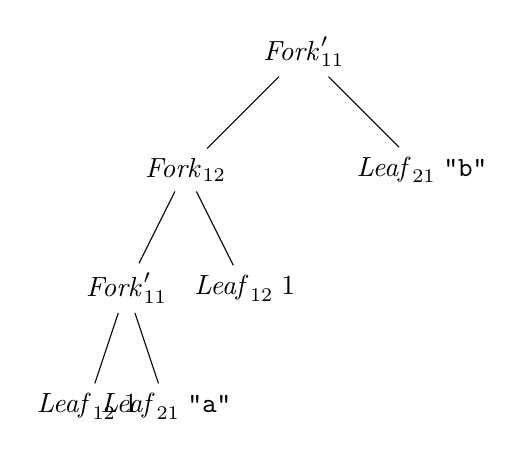
\begin{tikzpicture}[level/.style={sibling distance=30mm/#1}]
\node {\ensuremath{\Conid{Fork}_{11}'}}
  child {
      node {\ensuremath{\Conid{Fork}_{12}}}
          child {node {\ensuremath{\Conid{Fork}_{11}'}}
                    child {node {\ensuremath{\Conid{Leaf}_{12}\;\mathrm{1}}}}
                    child {node {\ensuremath{\Conid{Leaf}_{21}\;\text{\tt \char34 a\char34}}}}
          }
          child {node {\ensuremath{\Conid{Leaf}_{12}\;\mathrm{1}}}}
  }
  child {node {\ensuremath{\Conid{Leaf}_{21}\;\text{\tt \char34 b\char34}}}};
\end{tikzpicture}

\end{itemize}

\section{Zippers and dissections}
\label{sec:zippers-and-dissections}


\begin{itemize}
\item To lend more weight to the problem, show that
  zippers/derivatives, dissection, and infinitesimals are special
  cases (or possibly only some of these).
\end{itemize}

\section{Matrices of types}
\label{sec:matrices-of-types}

\begin{itemize}
\item Work up to the full solution involving matrices of types.
  Matrices!  Of types!
\end{itemize}

\section{Derivatives, again}
\label{sec:derivatives-again}

\begin{itemize}
\item Circle back round and discuss derivatives, dissection, and
  infinitesimals again from the new vantage point.  (e.g. discuss
  where the usual Leibniz equation comes from.)
\end{itemize}

\section{Divided differences}
\label{sec:divided-differences}

\begin{itemize}
\item Use the new power to also generalize dissections to divided
  differences.
\end{itemize}

\acks

Acknowledgments.

% We recommend abbrvnat bibliography style.

\bibliographystyle{abbrvnat}

\end{document}
